\documentclass[a4paper, 12pt]{article}

%\usepackage{cmap}
\usepackage[T2A]{fontenc}
\usepackage[utf8]{inputenc}
\usepackage[english, russian]{babel}
\usepackage{graphicx}
\usepackage[top=1in, bottom=1in, left=3.2cm, right=2.6cm]{geometry}
\graphicspath{./}
\usepackage{biblatex}
\addbibresource{lib.bib}
\linespread{1.5}

\usepackage{listings}
\usepackage{color}


\begin{document}
	
\begin{titlepage}
	\fontsize{12pt}{12pt}\selectfont
	\begin{figure}[t!]
		\centering
		
\includegraphics[scale=0.8]{bmstu}
	\end{figure}
	
	\noindent\rule{15cm}{3pt}
	\newline\newline
	\noindent 
	ФАКУЛЬТЕТ 
	\underline{«Информатика и системы управления»} \newline\newline
	
	\noindent КАФЕДРА \underline{«Программное обеспечение ЭВМ и информационные технологии»}\newline\newline\newline\newline\newline\newline
	
	\centering {\LARGE Отчет по лабораторной работе № 5}
	\vspace{3mm}
	
	\centering {\LARGE По курсу "Анализ Алгоритмов"
		\vspace{10mm}	
		
		\centering \bf Конвейерные вычисления}
	\vspace{10mm}
	
	
	\begin{flushright}
		{\large	Студент:\\ Турсунов Жасурбек Рустамович \\ Группа: ИУ7-56Б
			\vspace{5mm}
			\\Преподователи: \\ Волкова Лилия Леонидовна \\ Строганов Юрий Владимирович}
	\end{flushright}
	
	\begin{center}
		\vfill
		Москва, \the\year
		~г.
	\end{center}
\end{titlepage}

\tableofcontents
\clearpage
\newpage

\section*{Введение}

\begin{flushleft}
	\hspace*{5mm} Параллельные вычисления используют для увеличения скорости исполнения программ. Ведь пока нет возможности сделать один очень быстрый процессор, который можно было бы сравнить с современными параллельными компьютерами. Конвейерная обработка данных является популярным приемом при работе с параллельными машинами. 
	\newline \hspace*{5mm} В ходе лабораторной предстоит выполнить следующие задачи: 
	\begin{enumerate}
		\item изучение основ конвейерной обработки данных;
		\item получение практических навыков конвейерных вычислений;
		\item экспериментальное подтверждение различий во временной эффективности реализаций при помощи разработанного программного обеспечения на материале замеров процессорного времени выполнения;
		\item описание и обоснование полученных результатов в отчете о выполненной лабораторной работе.
	\end{enumerate}
	
\end{flushleft}
\clearpage
\newpage
\section{Аналитическая часть}
\begin{flushleft}
	\hspace*{5mm} В данной части будут рассмотрены главные принципы конвейерной обработки и параллельных вычислений.
	\subsection{Общие сведения о конвейерной обработке}
	\hspace*{5mm} {\bf Конвейер} - машина непрерывного транспорта, предназначенная для перемещения сыпучих, кусковых или штучных грузов.
	\\ \hspace*{5mm} {\bf Конвейерное производство} - система поточной организации производства на основе конвейера, при которой оно разделено на простейшие короткие операции, а перемещение деталей осуществляется автоматически. Это такая организация выполнения операций над объектами, при которой весь процесс воздействия разделяется на последовательность стадий с целью повышения производительности путём одновременного независимого выполнения операций над несколькими объектами, проходящими различные стадии. Конвейером также называют средство продвижения объектов между стадиями при такой организации.\cite{wiki}
	\\ \hspace*{5mm} Появилось в 1914 году на производстве Модели-Т на заводе Генри Форда и произвело революцию сначала в автомобилестроениии, а потом и во всей промышленности.
	\subsection{Параллельный алгоритм классического умножения матриц}
	\hspace*{5mm} Чтобы улучшить алгоритм, следует распараллелить ту часть алгоритма, которая содержит 3 вложенных цикла. Вычисление результата для каждой строки не зависит от результата выполнения умножения для других строк. Поэтому можно распараллелить часть кода, где происходят эти действия. Каждый поток будет выполнять вычисления определенных строк результирующей матрицы.
	\subsection{Параллельное программирование}
	\hspace*{5mm} При использовании многопроцессорных вычислительных систем с общей памятью обычно предполагается, что имеющиеся в составе системы процессоры обладают равной производительностью, являются равноправными при доступе к общей памяти, и время доступа к памяти является одинаковым (при одновременном доступе нескольких процессоров к одному и тому же элементу памяти очередность и синхронизация доступа обеспечивается на аппаратном уровне). Многопроцессорные системы подобного типа обычно именуются симметричными мультипроцессорами (symmetric multiprocessors, SMP).
	\\ \hspace*{5mm} Перечисленному выше набору предположений удовлетворяют также активно развиваемые в последнее время многоядерные процессоры, в которых каждое ядро представляет практически независимо функциони рующее вычислительное устройство. Для общности излагаемого учебного материала для упоминания одновременно и мультипроцессоров и много ядерных процессоров для обозначения одного вычислительного устройства.
	\\ \hspace*{5mm} Обычный подход при организации вычислений для многопроцессорных вычислительных систем с общей памятью – создание новых параллельных методов на основе обычных последовательных программ, в которых или автоматически компилятором, или непосредственно программистом выделяются участки независимых друг от друга вычислений. Возможности автоматического анализа программ для порождения параллельных вычислений достаточно ограничены, и второй подход является преобладающим. При этом для разработки параллельных программ могут применяться как новые алгоритмические языки, ориентированные на параллельное программирование, так и уже имеющиеся языки, расширенные некоторым набором операторов для параллельных вычислений.
	\\ \hspace*{5mm} Широко используемый подход состоит и в применении тех или иных библиотек, обеспечивающих определенный программный интерфейс (API) для разработки параллельных программ. В рамках такого подхода наиболее известны Windows Thread API. Однако первый способ применим только для ОС семейства Microsoft Windows, а второй вариант API является достаточно трудоемким для использования и имеет низкоуровневый характер. \cite{paral}
	\subsection{Организация взаимодействия параллельных потоков}
	\hspace*{5mm} Потоки исполняются в общем адресном пространстве параллельной программы. Как результат, взаимодействия параллельных потоков можно организовать через использование общих данных, являющихся доступными для всех потоков. Наиболее простая ситуация состоит в использовании общих данных только для чтения.
	\subsection{Описание метода}
	\hspace*{5mm} Конвейеризация - это техника, в результате которой задача разбивается на некоторое число подзадач, которые выполняются последовательно. Каждая подзадача выполняется на своем логическом устройстве. Все логические устройства соединяются последовательно таким образом, что выход i-ой ступени связан с выходом (i + 1)-ой ступени, все ступени работают одновременно. Множество ступеней называется конвейерном.
	\\ \hspace*{5mm} Выиграш во времени достигается при выполнении нескольких задач за счет параллельной работы ступеней, вовлекая на каждом такте новую задачу. Но в бесконвейерном подходе предсказать намного сложнее, и она может значительно различаться при разных данных.
	\subsection{Вывод}
	\hspace*{5mm} Были рассмотрены основы конвейерной обработки, технология параллельного программирования и организация взаимодействия параллельных потоков.
\end{flushleft}

\newpage
\section{Конструкторская часть}
\begin{flushleft}
	{\bf Требования к вводу: } Количество конвейеров должно быть больше 0.
	\\ {\bf Требования к программе при параллельной обработке: }
	\begin{enumerate}
		\item объекты должны последовательно проходить конвейеры в заданном порядке;
		\item конвейеры должны работать каждый в своем потоке; 
		\item конвейер должен завершать свою работу при поступлении специального элемента.
	\end{enumerate}

	\subsection{Организация обработки данных}
	\hspace*{5mm} На вход алгоритм получает одно число. Начальная функция пробрасывает число на уровень А. На уровне А, с помощью входного числа генерируются соответствующие числа для уровня В и пробрасываются в него. При этом уровень А начинает ожидать результата от уровня В. После его получения, числа суммируются в результат. Уровень В аналогичен уровню А - пробрасывает результат в С. Уровень С отправляет числа в функцию суммированию и возвращает результат в уровень В. На выходе получаем сумму чисел,  дошедших до уровня С. Все действия выполняются асинхронно. Функция суммирования работает в 9 потоков.\cite{geek} 
	
	\subsection{Вывод}
	\hspace*{5mm} В данном разделе была рассмотрена организация работы конвейерной обработки данных. Несмотря на сложность реализации многопоточной реализации, она даст выиграш, за счет параллельной обработки ресурсов. 
\end{flushleft}

\newpage
\section{Технологическая часть}
\begin{flushleft}
	\hspace*{5mm} В данном разделе будут рассмотрены требования к программному обеспечению, средства реализации и представлен листинг кода.
	\subsection{Требования к программному обеспечению}
		\begin{enumerate}
		\item программа должна корректно осуществлять передачу/прием между конвейерами;
		\item программа должна обеспечить возможность замера времени работы алгоритма. 
	\end{enumerate}
	\subsection{Средства реализации}
	\hspace*{5mm} В данной работе используется язык программирования Python, за высокую скорость выполнения программ и широкий выбор инструментов для параллельных вычислений. Проект выполнен в среде разработки Visual Studio Code. Многопоточное программирование было реализовано с помощью ThreadPoolExecutor. \cite{doc}
	\clearpage
	\newpage 
	\subsection{Листинг кода}
	В данном пункте представлен листинг кода, а именно:
	\begin{itemize}
		\item алгоритм конвейерной обработки данных.
	\end{itemize}
	\definecolor{codegreen}{rgb}{0,0.6,0}
	\definecolor{codegray}{rgb}{0.5,0.5,0.5}
	\definecolor{codepurple}{rgb}{0.58,0,0.82}
	\definecolor{backcolour}{rgb}{0.95,0.95,0.92}

	\lstdefinestyle{mystyle}{
		backgroundcolor=\color{backcolour},   
		commentstyle=\color{codegreen},
		keywordstyle=\color{magenta},
		numberstyle=\tiny\color{codegray},
		stringstyle=\color{codepurple},
		basicstyle=\ttfamily\footnotesize,
		breakatwhitespace=false,         
		breaklines=false,                 
		captionpos=b,                    
		keepspaces=true,                 
		numbers=left,                    
		numbersep=5pt,                  
		showspaces=false,                
		showstringspaces=false,
		showtabs=false,                  
		tabsize=4
	}

	\lstset{style=mystyle}

	\hspace*{5mm} На листинге 1 представлен код трехуровневого конвейера.
	\begin{lstlisting}[language=Python, caption = Конвейерный алгоритм]
	async def level_a(data):
		lvl_b_data = data, 2 * data, 4 * data
		results = await asyncio.gather(*[level_b(val) for val in lvl_b_data]) 
		result = await loop.run_in_executor(executor, cpu_bound_op, 3, *results)
		return result
		
		
	async def level_b(data):
		lvl_c_data = data, 3 * data, 5 * data
		results = await asyncio.gather(*[level_c(val) for val in lvl_c_data])
		result = await loop.run_in_executor(executor, cpu_bound_op, 2, *results)
		return result
		
		
	async def level_c(data):
		result = await loop.run_in_executor(executor, cpu_bound_op, 1, data)
		return result
	\end{lstlisting}
	
	\subsection{Вывод}
	\hspace*{5mm} В данном разделе была представлена структура ПО и листинги кода программы. 
	
\end{flushleft}

\newpage
\section{Исследовательская часть }
\begin{flushleft}
	\hspace*{5mm} В данном разделе будет проведен эксперимент и сравнительный анализ.
	\subsection{Системные характеристики}
	Характеристики компьютера на котором проводился замер времени сортировки массива:
	\begin{enumerate}
		\item операционная система - Windows 10;
		\item процессор - Intel(R) Core(TM) i7-10510U CPU @1.80GHz 2.30GHz;
		\item оперативная память - 16 ГБ;
		\item количество ядер - 4;
		\item количество логических процессов - 8.
	\end{enumerate}
	\subsection{Постановка эксперимента}
	В рамках данного проекта были проведены эксперименты, описанные ниже:
	\begin{enumerate}
		\item сравнение и анализ времени работы конвейера для разного количества потоков;
		\item сравнение и анализ времени работы программы при асинхронном и не асинхронном программировании.
	\end{enumerate}
	\clearpage
	\newpage
	\subsection{Сравнительный анализ на основе замеров времени работы программы}
	Был проведен замер времени работы каждого потока.
	\\ \hspace*{5mm} На рисунке 1 показаны результаты первого эксперимента, суть которого заключается в анализе зависимости числа потоков от времени работы конвейра при одном и том же числовом значении. Ниже приведена полученная диаграмма:
	\begin{figure}[h]
		\centering 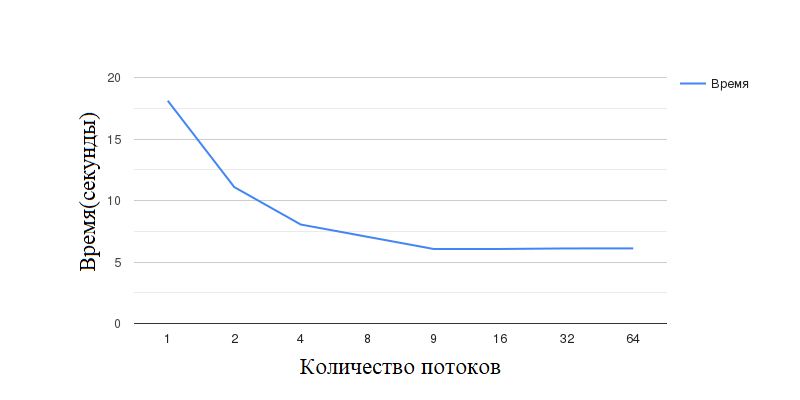
\includegraphics[scale=2]{chart (1)}
		\centering\caption{Сравнение времени работы конвейера при разном количестве потоков}
	\end{figure}
	
	\hspace*{5mm}  На рисунке 2 показаны результаты первого эксперимента, суть которого заключается в анализе зависимости числа потоков от времени работы процессора при одном и том же числовом значении. Ниже приведена полученная диаграмма:
	\clearpage
	\newpage 
	\begin{figure}[h]
		\centering 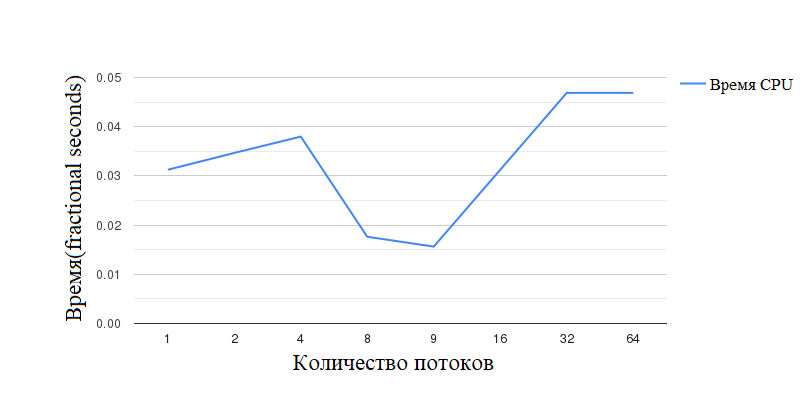
\includegraphics[scale=2]{chart (2)}
		\centering\caption{Сравнение времени работы процессора при работе конвейера при разном количестве потоков.}
	\end{figure}
	\hspace*{5mm} Третий эксперимент был проведен, для того чтобы сделать анализ зависимости времени работы при асинхронном и не асинхронном программировании. В таблице 1 показаны результаты этого эксперимента.
	\newline \\
	\begin{table}[h]
		\centering
		\caption{Результаты временного замери при асинхронном и не асинхронном программировании.\\}
		\begin{tabular}{ | c | c | c | }
			\hline
			Входное число & Асинхронно & Не асинхронно  \\ \hline
			2 & 6.052519 | 0.015625 & 18.024558 | 0.015625 \\ \hline
			100 & 6.051918 | 0.015625 & 18.010213 | 0.015625  \\ \hline
			10 000 & 6.055719 | 0.031250 & 18.009668 | 0.015600 \\ \hline
			10 000 000 & 6.061437 | 0.031250 & 18.003867 | 0.015534  \\ 
			\hline
		\end{tabular}
	\end{table}

	\clearpage
	\newpage
	\subsection{Вывод}
	\hspace*{5mm} По проведенному анализу из первого эксперимента можно сделать вывод, что наилучшее время работы было достигнуто, когда количество потоков равно 9. Это не случайный результат, потому что на уровне С выполняется 9 вычислений. Следовательно у каждого потока была своя задача и так как у нас не было лишних или недостающих потоков и был достигнут такой результат. Второй эксперимент был отчасти связан с первым. Единственным отличием было замер времени. Здесь он проводился у самого процессора. Сделав небольшой анализ, можно понять, что лучший результат был достигнут когда количество потоков было равным 9. Третий эксперимент был проведен чтобы увидеть значимую разницу при асинхронном и не асинхронном программировании. Асинхронный метод с конвейерной реализацией показал время в три раза быстрее чем при не асинхронном методе, что не скажешь про время работы самого процессора. Лучший показатель был достигнкт при не асинхронном методе и без конвейера. 
\end{flushleft}

\begin{flushleft}
	\newpage
	\section*{Заключение}
	\hspace*{5mm} В рамках данной работы успешно изучены основы контейнерных вычислений. Применен метод асинхронного и не асинхронного программирования. Проведен сравнительный анализ контейнерной и традиционной реализаций. Подтверждены экспериментально различия во временной эффективности реализаций при помощи разработанного программного обеспечения на материале замеров времени выполнения в зависимости от загруженности процесса. Дано описание и обоснование полученных результатов.
	\\ \hspace*{5mm} Экспериментально получено, что реализация с контейнерами работает более чем три раза быстрее, нежели традиционная.   
\end{flushleft}

\clearpage
\newpage

\printbibliography

\end{document}